%%%%%%%%%%%%%%%%%%%%%%%%%%%%%%%%%%%%%%%%%%%%%%%%%%%%%%%%%%%%%%%%%%%%%%%%%%%%%%%%%%
\begin{frame}[fragile]\frametitle{}
\begin{center}
{\Large Building a Chatbot: A Walk-through}

{\tiny (Ref:``Building a Conversational Chatbot for Slack using Rasa and Python'' - Parul Pandey, which in turn is based on Pydata Berlin talk by Tom Bocklisch )}
\end{center}
\end{frame}

%%%%%%%%%%%%%%%%%%%%%%%%%%%%%%%%%%%%%%%%%%%%%%%%%%%%%%%%%%%
 \begin{frame}[fragile]\frametitle{Objective}
   \begin{columns}
    \begin{column}[t]{0.5\linewidth}
\begin{itemize}
\item To build a chatbot called ‘Robo’
\item Capable of checking in on people’s mood and taking the necessary actions to cheer them up.
\item Deployment on Slack 
\end{itemize}
    \end{column}
    \begin{column}[t]{0.5\linewidth}
\begin{center}
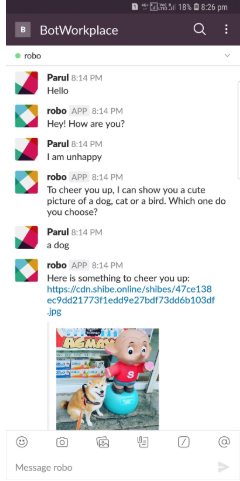
\includegraphics[width=0.6\linewidth,keepaspectratio]{chatbot2}
\end{center}
    \end{column}
  \end{columns}
\end{frame}



%%%%%%%%%%%%%%%%%%%%%%%%%%%%%%%%%%%%%%%%%%%%%%%%%%%%%%%%%%%
 \begin{frame}[fragile]\frametitle{Rasa NLU Training}
   \begin{columns}
    \begin{column}[t]{0.5\linewidth}
\begin{itemize}
\item Teaching how to understand user inputs, extract intent and entities
\item Need to build a Rasa NLU model and feed in the training data which the user has to prepare.
\item Using model, any user input can then predict intent and entities.
\end{itemize}
    \end{column}
    \begin{column}[t]{0.5\linewidth}
\begin{center}
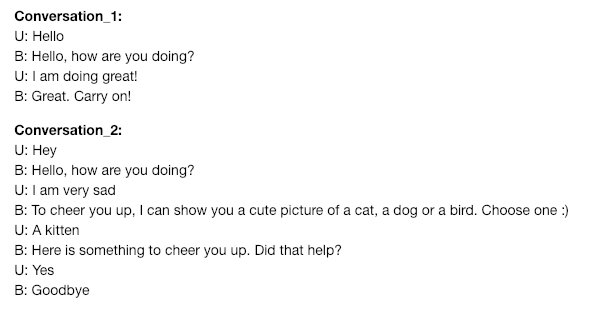
\includegraphics[width=\linewidth,keepaspectratio]{chatbot4}
\end{center}
    \end{column}
  \end{columns}
\end{frame}

%%%%%%%%%%%%%%%%%%%%%%%%%%%%%%%%%%%%%%%%%%%%%%%%%%%%%%%%%%%
 \begin{frame}[fragile]\frametitle{NLU training file}
 nlu.md

\begin{lstlisting}
## intent:greet
- hey
- hello there
- hi
- hello there
## intent:goodbye
- cu
- good by
- cee you later
## intent:mood_unhappy
- my day was horrible
- I am sad
- I don't feel very well
- I am disappointed
\end{lstlisting}

You can also add some spelling mistakes or slangs since that will give a flavour of the spoken language to the bot.

\end{frame}

%%%%%%%%%%%%%%%%%%%%%%%%%%%%%%%%%%%%%%%%%%%%%%%%%%%%%%%%%%%
 \begin{frame}[fragile]\frametitle{Defining the NLU Model Configuration}
config.yml

\begin{lstlisting}
language: "en"

pipeline:
- name: "nlp_spacy"                   # loads the spacy language model
- name: "tokenizer_spacy"             # splits the sentence into tokens
- name: "ner_crf"                   # uses the pretrained spacy NER model
- name: "intent_featurizer_spacy"     # transform the sentence into a vector representation
- name: "intent_classifier_sklearn"   # uses the vector representation to classify using SVM
- name: "ner_synonyms"                # trains the synonyms
\end{lstlisting}

\begin{itemize}
\item Rasa NLU has a number of different components, which together make a pipeline. 
\item Once the training data is ready, we can feed it to the NLU model pipeline. 
\item All the components that are listed in the pipeline will be trained one after another.
\end{itemize}

\end{frame}

%%%%%%%%%%%%%%%%%%%%%%%%%%%%%%%%%%%%%%%%%%%%%%%%%%%%%%%%%%%
 \begin{frame}[fragile]\frametitle{Training the NLU Model}
\begin{lstlisting}
from rasa_nlu.training_data import load_data
from rasa_nlu.config import RasaNLUModelConfig
from rasa_nlu.model import Trainer
from rasa_nlu import config

training_data = load_data("nlu.md")
trainer = Trainer(config.load("config.yml"))
interpreter = trainer.train(training_data)
model_directory = trainer.persist("./models/nlu", fixed_model_name="current")
\end{lstlisting}

When you send a message like “hello” to your bot, it will recognise this as a greet intent and when you send ‘bye’, it recognises it as a goodbye intent. The trained model files will be stored at path: ‘./models/nlu/current’.

\end{frame}

%%%%%%%%%%%%%%%%%%%%%%%%%%%%%%%%%%%%%%%%%%%%%%%%%%%%%%%%%%%
 \begin{frame}[fragile]\frametitle{Evaluating the NLU model}
 
    \begin{columns}
    \begin{column}[t]{0.5\linewidth}
	 Let's test how our model performs. Let’s pass in some random messages.

\begin{lstlisting}
# small helper to make dict dumps a bit prettier
def pprint(o):
   print(json.dumps(o, indent=2))
pprint(interpreter.parse("I am unhappy"))
\end{lstlisting}
    \end{column}
    \begin{column}[t]{0.5\linewidth}
\begin{center}
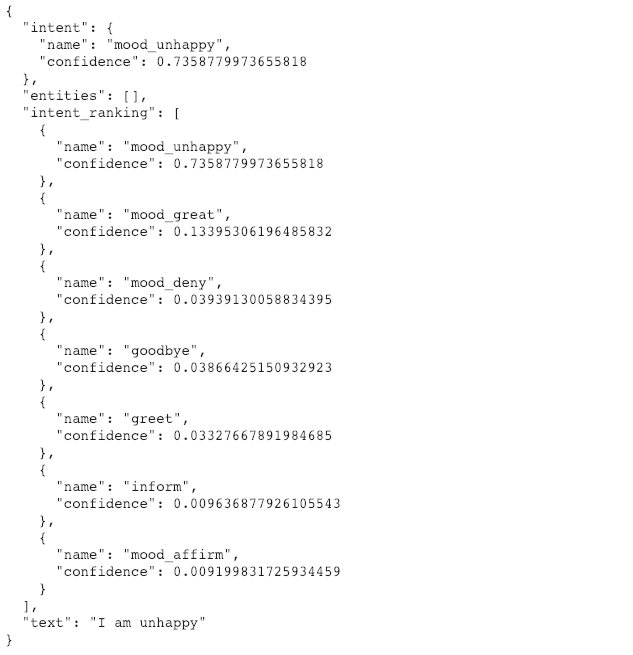
\includegraphics[width=\linewidth,keepaspectratio]{chatbot7}
\end{center}

Our model has performed well. 
    \end{column}
  \end{columns}
\end{frame}

%%%%%%%%%%%%%%%%%%%%%%%%%%%%%%%%%%%%%%%%%%%%%%%%%%%%%%%%%%%
 \begin{frame}[fragile]\frametitle{Evaluating the NLU model}
 
    \begin{columns}
    \begin{column}[t]{0.5\linewidth}
Let us now evaluate it on a test data set. However, for our purpose let’s evaluate it on the data at hand i.e nlu.md
\begin{lstlisting}
from rasa_nlu.evaluate import run_evaluation
run_evaluation("nlu.md", model_directory)
\end{lstlisting}

We get an Intent Confusion matrix with the with various evaluation results.
    \end{column}
    \begin{column}[t]{0.5\linewidth}
\begin{center}
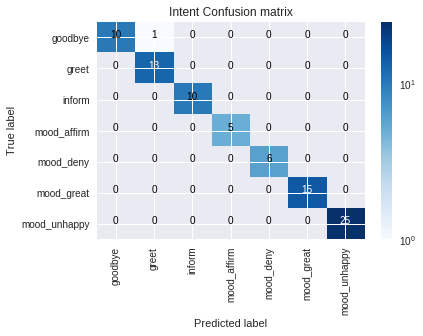
\includegraphics[width=\linewidth,keepaspectratio]{chatbot8}
\end{center}
    \end{column}
  \end{columns}
\end{frame}

%%%%%%%%%%%%%%%%%%%%%%%%%%%%%%%%%%%%%%%%%%%%%%%%%%%%%%%%%%%
 \begin{frame}[fragile]\frametitle{Evaluating the NLU model}
 
    \begin{columns}
    \begin{column}[t]{0.5\linewidth}
\begin{itemize}
\item We have successfully created a basic Bot
\item It is now capable of understanding what the user is saying i.e whether is our mood like, is it happy or sad. 
\item But it has no dialogues. 
\item Now the next task would be to make the Bot respond to messages.
\end{itemize}
    \end{column}
    \begin{column}[t]{0.5\linewidth}
\begin{center}
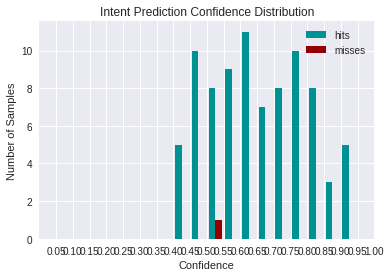
\includegraphics[width=0.6\linewidth,keepaspectratio]{chatbot9}
\end{center}
    \end{column}
  \end{columns}
\end{frame}

%%%%%%%%%%%%%%%%%%%%%%%%%%%%%%%%%%%%%%%%%%%%%%%%%%%%%%%%%%%
 \begin{frame}[fragile]\frametitle{Teaching the bot to respond using Rasa Core}

\begin{itemize}
\item For responding to a message, it would be to fetch an image of a dog, cat or a bird depending upon user’s choice to cheer them up. 
\item We will teach ‘robo’ to make responses by training a dialogue management model using Rasa Core.
\item For dialog training, Rasa has 4 main components
\begin{itemize}
\item Domain(domain.yml)
\item Stories (stories.md)
\item Policies (policy.yml)
\item Custom Actions (actions.py)
\end{itemize}

\end{itemize}
\end{frame}


%%%%%%%%%%%%%%%%%%%%%%%%%%%%%%%%%%%%%%%%%%%%%%%%%%%%%%%%%%%
 \begin{frame}[fragile]\frametitle{Defining a Domain}

\begin{itemize}
\item The domain is like a universe where the bot lives in operates. 
\item This includes what user inputs it should expect to get, what actions it should be able to predict, how to respond and what information to store. 
\item The domain consists of five key parts consisting of intents, slots, entities, actions and templates
\item slots: slots are like placeholders for the values that enable the bot to keep a track of the conversations.
\item actions: things our bot would say or do.
\item templates: template strings for the things that bot would say
\item We define the domain in form of a domain.yml life
\end{itemize}
\end{frame}

%%%%%%%%%%%%%%%%%%%%%%%%%%%%%%%%%%%%%%%%%%%%%%%%%%%%%%%%%%%
 \begin{frame}[fragile]\frametitle{Defining a Domain}
Here is an example domain for our bot: 

domain.yml

\begin{lstlisting}
intents:
- greet
- goodbye
- mood_affirm

slots:
  group:
    type: text
    
entities:
- group

actions:
- utter_greet
- utter_did_that_help
- utter_happy

\end{lstlisting}

domain.yml to be continued \ldots
\end{frame}

%%%%%%%%%%%%%%%%%%%%%%%%%%%%%%%%%%%%%%%%%%%%%%%%%%%%%%%%%%%
 \begin{frame}[fragile]\frametitle{Defining a Domain}
domain.yml

\begin{lstlisting}
templates:
  utter_greet:
  - text: "Hey! How are you?"
  
utter_goodbye:
  - text: "Bye"
  
  utter_ask_picture:
  - text: "To cheer you up, I can show you a cute picture of a dog, cat or a bird. Which one do you choose?"
\end{lstlisting}

\end{frame}

%%%%%%%%%%%%%%%%%%%%%%%%%%%%%%%%%%%%%%%%%%%%%%%%%%%%%%%%%%%
 \begin{frame}[fragile]\frametitle{Defining a Domain}

\begin{itemize}
\item If you see we have defined a slot which would help bot to have some memory about the conversation. 
\item All entities and intents are mentioned. 
\item We have defined some actions and templates also for the bot to respond to user messages. 
\item In actions, there are utter actions (utter\_greet, \ldots) and custom actions (utter\_ask\_picture). 
\item ‘utter\_default’ can be used for a fallback in case bot is not able to understand the user message.
\end{itemize}

\end{frame}


%%%%%%%%%%%%%%%%%%%%%%%%%%%%%%%%%%%%%%%%%%%%%%%%%%%%%%%%%%%
 \begin{frame}[fragile]\frametitle{Writing Stories}

\begin{itemize}
\item Once we have defined our domain now let’s create a sample user-bot interaction.
\item The training data for dialogue management models is called stories. 
\item A story consist of an actual piece of conversation that takes place between a user and Bot. 
\item The user’s inputs are expressed as intents as well as corresponding entities, and chatbot responses are expressed as actions.
\end{itemize}
\end{frame}

%%%%%%%%%%%%%%%%%%%%%%%%%%%%%%%%%%%%%%%%%%%%%%%%%%%%%%%%%%%
 \begin{frame}[fragile]\frametitle{Writing Stories}
 Let’s see how a typical story looks like.
 
 
    \begin{columns}
    \begin{column}[t]{0.5\linewidth}
	 stories.md

\begin{lstlisting}
## happy path               
* greet              
  - utter_greet
* mood_great              
  - utter_happy
* mood_affirm
  - utter_happy
* mood_affirm
  - utter_goodbye
  
## sad path          
* greet
  - utter_greet             
* mood_unhappy
  - utter_ask_picture
* inform{"animal":"dog"}  
  - action_retrieve_image
  - utter_did_that_help
* mood_affirm
  - utter_happy
\end{lstlisting}
    \end{column}
    \begin{column}[t]{0.5\linewidth}
	Syntax:
\begin{itemize}
\item \#\# denotes the start of a story and you can give it a name like happy path, sad path etc.
\item * denotes the messages sent by the user in the form of intents.
\item - denotes the action taken by the bot
\end{itemize}

So if you see above, We have defined various paths for the user and bot conversation. Always good to have more stories to train the dialog better.

    \end{column}
  \end{columns}
\end{frame}


%%%%%%%%%%%%%%%%%%%%%%%%%%%%%%%%%%%%%%%%%%%%%%%%%%%%%%%%%%%
 \begin{frame}[fragile]\frametitle{Policies}

\begin{itemize}
\item The rasa core policies decide which action to take at every step in the conversation. 
\item There are different policies to choose from, and one can include multiple policies in a single rasa core Agent but at every turn, the policy which predicts the next action with the highest confidence will be used. 
\item We have configured a basic policy(policy.yml) for our bot as shown below which has FallbackPolicy as well. 
\item The fallback policy comes in to picture when ‘nlu\_threshold’ \& ‘core\_threshold’ meets the levels defined in the policy which means that bot is not able to understand the user message and it responds with ‘utter\_default’.
\end{itemize}
\end{frame}

%%%%%%%%%%%%%%%%%%%%%%%%%%%%%%%%%%%%%%%%%%%%%%%%%%%%%%%%%%%
 \begin{frame}[fragile]\frametitle{Policies}

 policy.yml
 
 
\begin{lstlisting}
policies:
  - name: KerasPolicy
    epochs: 100
    max_history: 3
  - name: MemoizationPolicy
    max_history: 3
  - name: FallbackPolicy
    nlu_threshold: 0.1
    core_threshold: 0.2
    fallback_action_name: 'utter_default'
  - name: FormPolicy
\end{lstlisting}

\end{frame}

%%%%%%%%%%%%%%%%%%%%%%%%%%%%%%%%%%%%%%%%%%%%%%%%%%%%%%%%%%%
 \begin{frame}[fragile]\frametitle{Custom Actions}

  
\begin{itemize}
\item We have already defined the utter action by adding an utterance template to the domain file but if we need to run any code we want then we would need custom actions. 
\item Custom actions can do anything that you can imagine like turning on the lights, adding an event to a calendar, check a user’s bank balance, etc.
\item Since we want our Bot to make an API call to retrieve photographs of a dog, cat or a bird, depending on which was specified by the user, we need to create a custom action. 
\item The bot will know which type of picture should be received by retrieving the value of the slot group
\end{itemize}

\end{frame}

% %%%%%%%%%%%%%%%%%%%%%%%%%%%%%%%%%%%%%%%%%%%%%%%%%%%%%%%%%%%
 % \begin{frame}[fragile]\frametitle{Custom Actions}

  
% \begin{itemize}
% \item Rasa Core calls an endpoint specified by us when a custom action is predicted. 
% \item This endpoint should be a web server that reacts to this call, runs the code and optionally returns information to modify the dialogue state.
% \item 
% To specify, our action server we use the endpoints.yml and pass it to the scripts using \lstinline|--endpoints endpoints.yml|

% \begin{lstlisting}
% action_endpoint:
  % url: "http://localhost:5055/webhook"
% \end{lstlisting}
% \item Though we can create an action server in node.js, .NET, Java, or any other language and define our actions there, but Rasa has provided a small python sdk to make the things easier for us.
% \begin{lstlisting}
% pip install rasa_core_sdk
% \end{lstlisting}
% \end{itemize}





% \end{frame}


%%%%%%%%%%%%%%%%%%%%%%%%%%%%%%%%%%%%%%%%%%%%%%%%%%%%%%%%%%%
 \begin{frame}[fragile]\frametitle{Custom Actions}

 actions.py

  
\begin{lstlisting}
from rasa_core.actions import Action
from rasa_core.events import SlotSet
from IPython.core.display import Image, display

import requests

class ApiAction(Action):
    def name(self):
        return "action_retrieve_image"

    def run(self, dispatcher, tracker, domain):
        
        group = tracker.get_slot('group')
        url = 'http://shibe.online/api/{}?count=1&urls=true&httpsUrls=true'
        r = requests.get(url.format(group))
        response = r.content.decode()
        response = response.replace('["',"")
        response = response.replace('"]',"")
		message = "Here is something to cheer you up: {}"
        #display(Image(response[0], height=550, width=520))
        dispatcher.utter_message(message.format(response))
\end{lstlisting}

\end{frame}


%%%%%%%%%%%%%%%%%%%%%%%%%%%%%%%%%%%%%%%%%%%%%%%%%%%%%%%%%%%
 \begin{frame}[fragile]\frametitle{Training a Dialogue Model}

\begin{itemize}
\item Finally, we will train the dialogue management model citing the policies that should be used to train it. 
\item For our example, we will implement a neural network in Keras which learns to predict which action to take next.
\item The main component of the model is a recurrent neural network (an LSTM), which maps from raw dialogue history directly to distribution over system actions.
\end{itemize}

\end{frame}

%%%%%%%%%%%%%%%%%%%%%%%%%%%%%%%%%%%%%%%%%%%%%%%%%%%%%%%%%%%
 \begin{frame}[fragile]\frametitle{Training a Dialogue Model}

\begin{lstlisting}
from rasa_core.policies import FallbackPolicy, KerasPolicy, MemoizationPolicy
from rasa_core.agent import Agent

# The fallback action will be executed if the intent recognition has #a confidence below nlu_threshold or if none of the dialogue #policies predict an action with confidence higher than #core_threshold.

fallback = FallbackPolicy(fallback_action_name="utter_unclear",
                          core_threshold=0.2,
                          nlu_threshold=0.1)

agent = Agent('domain.yml', policies=[MemoizationPolicy(), KerasPolicy(), fallback])

# loading our neatly defined training dialogues
training_data = agent.load_data('stories.md')

agent.train(training_data)

agent.persist('models/dialogue')
\end{lstlisting}

\end{frame}

%%%%%%%%%%%%%%%%%%%%%%%%%%%%%%%%%%%%%%%%%%%%%%%%%%%%%%%%%%%
 \begin{frame}[fragile]\frametitle{Training a Dialogue Model}

Sometimes you want to fall back to a fallback action like saying “Sorry, I didn’t understand that”. To do this, add the FallbackPolicy to your policy ensemble.

\begin{center}
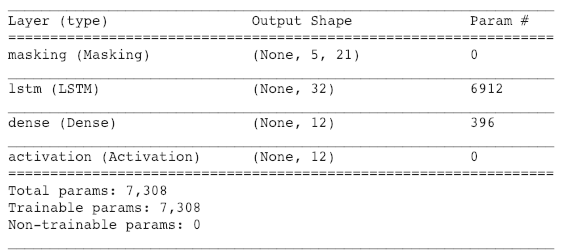
\includegraphics[width=0.8\linewidth,keepaspectratio]{chatbot10}
\end{center}

The model will be saved at the path :‘models/dialogue’

\end{frame}

%%%%%%%%%%%%%%%%%%%%%%%%%%%%%%%%%%%%%%%%%%%%%%%%%%%%%%%%%%%
 \begin{frame}[fragile]\frametitle{ Time to chat}

\begin{lstlisting}
import warnings
warnings.simplefilter('ignore', ruamel.yaml.error.UnsafeLoaderWarning)
from rasa_core.agent import Agent
from rasa_core.interpreter import NaturalLanguageInterpreter
interpreter = NaturalLanguageInterpreter.create(model_directory)
agent = Agent.load('models/dialogue', interpreter=interpreter)
print("Your bot is ready to talk! Type your messages here or send 'stop'")
while True:
    a = input()
    if a == 'stop':
        break
    responses = agent.handle_text(a)
    for response in responses:
        print(response["text"])
\end{lstlisting}

\end{frame}

%%%%%%%%%%%%%%%%%%%%%%%%%%%%%%%%%%%%%%%%%%%%%%%%%%%%%%%%%%%%%%%%%%%%%%%%%%%%%%%%%%
\begin{frame}[fragile]\frametitle{}
\begin{center}
{\Large Deployment on Slack (Optional)}

\end{center}
\end{frame}


%%%%%%%%%%%%%%%%%%%%%%%%%%%%%%%%%%%%%%%%%%%%%%%%%%%%%%%%%%%
 \begin{frame}[fragile]\frametitle{Deployment on Slack}
Let’s us create a slack integration by creating a slack app. 

\begin{itemize}
\item Create a Slack account and go to https://api.slack.com/. 
\item Now choose either an existing development Slack workplace(in case you have one) or create a new one. Name it DemoWorkplace or anything you like.
\item Now create a Slack app in DemoWorkplace and give it a name. Let’s call our app Robo.
\end{itemize}

\end{frame}

%%%%%%%%%%%%%%%%%%%%%%%%%%%%%%%%%%%%%%%%%%%%%%%%%%%%%%%%%%%
 \begin{frame}[fragile]\frametitle{Deployment on Slack}
Start adding features and functionalities to the app


\begin{itemize}
\item First create a bot user under the Bots Tab and integrate it into the app. 
\item This will make the app conversational. 
\item Since this bot will be created as a user, we can choose to keep it constantly online. 
\item Save all the changes made.
\end{itemize}

\end{frame}


%%%%%%%%%%%%%%%%%%%%%%%%%%%%%%%%%%%%%%%%%%%%%%%%%%%%%%%%%%%
 \begin{frame}[fragile]\frametitle{Deployment on Slack}
To make sure that the bot has been integrated:

\begin{itemize}
\item Navigate to the Add Features and Functionality under Basic Information Tab and make sure that the Bots and Permissions Tabs are active. Our bot has been integrated into the app.
\item Next, we can add a lit bit more info about our bot including a picture, a description and a background colour. 
\item Scroll to Display Information and add in the information.
\item Save all changes as you go.
\end{itemize}

\end{frame}

%%%%%%%%%%%%%%%%%%%%%%%%%%%%%%%%%%%%%%%%%%%%%%%%%%%%%%%%%%%
 \begin{frame}[fragile]\frametitle{Deployment on Slack}

\begin{itemize}
\item Lastly, we need to install this app into our workplace which we defined earlier. 
\item Authorize it and we have our app ready and integrated into the workplace.
\end{itemize}

\end{frame}

%%%%%%%%%%%%%%%%%%%%%%%%%%%%%%%%%%%%%%%%%%%%%%%%%%%%%%%%%%%
 \begin{frame}[fragile]\frametitle{Ngrok}

\begin{itemize}
\item Opens access to your local app from the internet.
\item Download ngrok from https://dashboard.ngrok.com/get-started. make sure you Login first.
\item Unzip to install via \lstinline|$ unzip /path/to/ngrok.zip|
\item Connect your account via \lstinline|$ ./ngrok <authtoken>$|
\item The token can be accessed from https://dashboard.ngrok.com/auth.
\item Start it by telling it which port we want to expose to the public internet : \lstinline|./ngrok http 5004|
\end{itemize}

\begin{center}
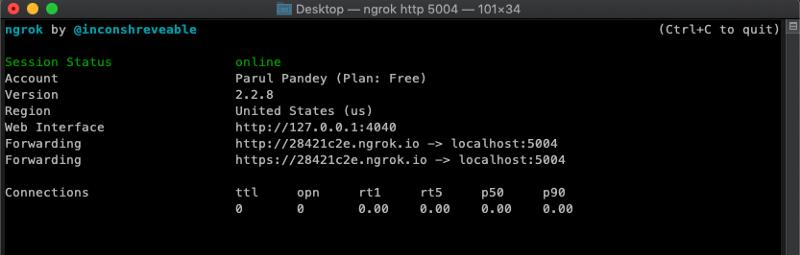
\includegraphics[width=0.8\linewidth,keepaspectratio]{chatbot11}
\end{center}
\end{frame}

%%%%%%%%%%%%%%%%%%%%%%%%%%%%%%%%%%%%%%%%%%%%%%%%%%%%%%%%%%%
 \begin{frame}[fragile]\frametitle{Create a Python Script}

\begin{itemize}
\item Create run\_app.py to integrate our chatbot with the slack app 
\item We will begin by creating a slack connector for our Rasa chatbot. 
\item We will use RasaNLU interpreter to load the NLU model directly from the python script.
\end{itemize}

\end{frame}

%%%%%%%%%%%%%%%%%%%%%%%%%%%%%%%%%%%%%%%%%%%%%%%%%%%%%%%%%%%
 \begin{frame}[fragile]\frametitle{Training}

\begin{itemize}
\item Training the NLU Model \lstinline|python nlu_model.py|
\item Start the custom action server \lstinline|python -m rasa_core_sdk.endpoint --actions actions|
\item Open a new terminal and train the Rasa Core model \lstinline|python dialogue_management_model.py|
\item Start the Agent by running run\_app.py Make sure to provide the slack token in the script.
\end{itemize}

\end{frame}

%%%%%%%%%%%%%%%%%%%%%%%%%%%%%%%%%%%%%%%%%%%%%%%%%%%%%%%%%%%
 \begin{frame}[fragile]\frametitle{Connections}

\begin{itemize}
\item Start the ngrok on port 5004 and grab your ngrok\_url.
\item Provide the url: https://<your\_ngrok\_url>/webhooks/slack/webhook to ‘Event Subscriptions’ page of the Slack configuration. Wait for it to be verified.
\item Lastly, subscribe to some Workplace events like
\begin{itemize}
\item app\_mention so that our bot responds when someone mentions it by name
\item message\_im which allows the user to send direct messages to the bot.
\end{itemize}
\item Make sure to save all the changes as you go
\end{itemize}

\end{frame}
%%%%%%%%%%%%%%%%%%%%%%%%%%%%%%%%%%%%%%%%%%%%%%%%%%%%%%%%%%%
 \begin{frame}[fragile]\frametitle{Let’s Talk}

\begin{itemize}
\item Ensure the custom actions server is running
\item Ensure ngrok is running on port 5004
\item Navigate to Slack interface and talk to your bot
\end{itemize}

\begin{center}
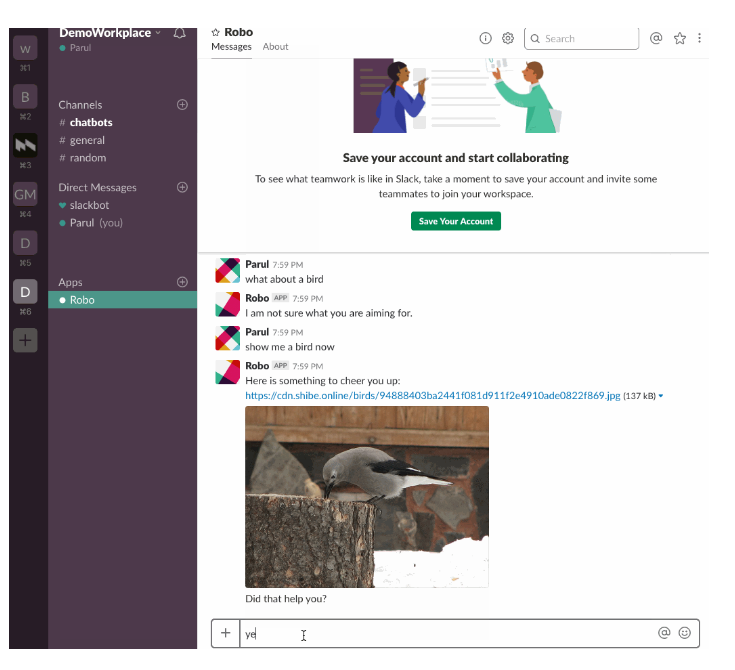
\includegraphics[width=0.6\linewidth,keepaspectratio]{chatbot12}
\end{center}
\end{frame}

%%%%%%%%%%%%%%%%%%%%%%%%%%%%%%%%%%%%%%%%%%%%%%%%%%%%%%%%%%%
 \begin{frame}[fragile]\frametitle{Conclusion}

\begin{itemize}
\item We created a chatbot which is capable of listening to user’s input and responding contextually.
\item We utilised the capabilities of Rasa NLU and Rasa Core to create a bot with minimum training data. 
\end{itemize}

\end{frame}